\title{ }
\author{
        Justin Baraboo \\
         Design and Analysis of Algorithms\\
        Assignment 4\\
       }


\documentclass[12pt]{article}
\usepackage{amsmath}
\usepackage[pdftex]{graphicx}
\usepackage{listings}
\usepackage{color}

\usepackage{pgf}
\usepackage{tikz}
\usetikzlibrary{arrows,automata}


\definecolor{dkgreen}{rgb}{0,0.6,0}
\definecolor{gray}{rgb}{0.5,0.5,0.5}
\definecolor{mauve}{rgb}{0.58,0,0.82}

\lstset{frame=tb,
  language=Java,
  aboveskip=3mm,
  belowskip=3mm,
  showstringspaces=false,
  columns=flexible,
  basicstyle={\small\ttfamily},
  numbers=none,
  numberstyle=\tiny\color{gray},
  keywordstyle=\color{blue},
  commentstyle=\color{dkgreen},
  stringstyle=\color{mauve},
  breaklines=true,
  breakatwhitespace=true,
  tabsize=3
}

\begin{document}
\maketitle


\section{Problem 1}
Conduct a DFS for the following graph.\\


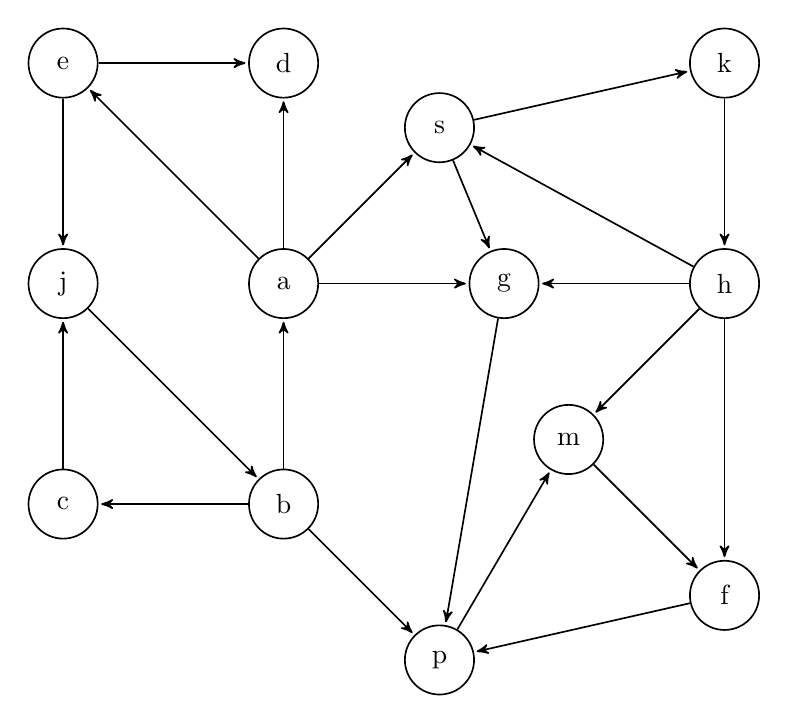
\begin{tikzpicture}[->,>=stealth',shorten >=1pt,auto,node distance=2.8cm,
                    semithick]
%  \tikzstyle{every state}=[fill=white,draw=none,text=black]

  \node[state]         (E)                                {e};
  \node[state]         (D) [ right of=E] {d};
  \node[state]         (A) [below of= D] {a};
  \node[state]         (J) [below of =E] {j};
  \node[state]         (C) [below of=J]          {c};
  \node[state]         (B) [below of=A]  {b};
  \node[state]         (G) [right of=A]       {g};
  \node[state]         (S) [above right of = A] {s};
  \node[state]         (P) [below right of=B] {p};
  \node[state]         (H) [right of = G] {h};
  \node[state]         (M) [below left of=H] {m};
  \node[state]         (K) [above of=H]          {k};
  \node[state]         (F) [below right of=M]  {f};


  \path (A) edge              node {} (D)
                  edge              node {} (E)
                  edge              node {} (G)
    	       edge              node {} (S)
        (B) edge                  node {} (A)
            edge                    node {} (C)
	 edge                    node {} (P)
        (C) edge                  node {} (J)
        (E) edge                  node {} (D)
              edge                  node {} (J)
         (F) edge                 node {} (P)
        (G) edge                  node {} (P)
        (H) edge                  node {} (S)
              edge                    node {} (G)
              edge                    node {} (M)
              edge                    node {} (F)
        (J) edge                  node {} (B)
        (K) edge                  node {} (H)
         (M) edge                 node {} (F)
         (P) edge                 node {} (M)
         (S) edge                 node {} (G)
               edge                 node {} (K)
;
\end{tikzpicture}


\paragraph{Solution}

For our DFS, we start at node $a$, we then go to node $d$ which has no neighbors so we go to back to $a$.\\
We then go to $e$ then from there to $j$, $b$, $c$ where we have no node to go to. So we go back to $b$.\\
From there we go to $p$, $m$, $f$.Where we find no nodes to go to.  We go back through our visited nodes finding they have no more nodes to visit until we reach back to $a$.\\
We then go to $g$ find no node to visit and go back to $a$.  We then go to $s$, then to $k$ and then to $h$ and we find no nodes to visit.  We go back through and find no nodes
to visit for any of our nodes.  We then realize we have traversed the graph and are done.\\
\\

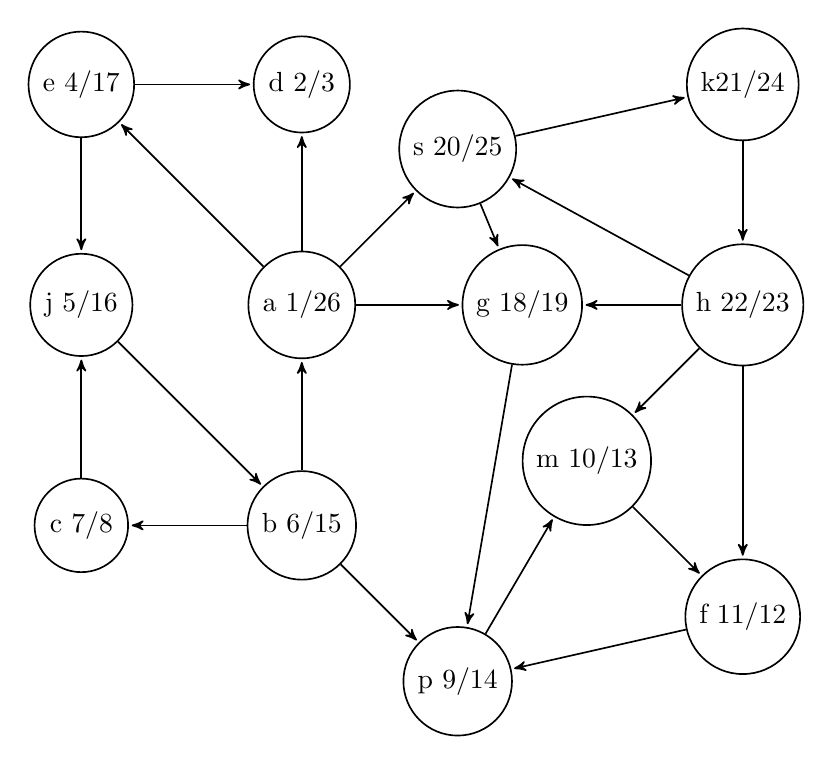
\begin{tikzpicture}[->,>=stealth',shorten >=1pt,auto,node distance=2.8cm,
                    semithick]
%  \tikzstyle{every state}=[fill=white,draw=none,text=black]

  \node[state]         (E)                                {e $4/17$};
  \node[state]         (D) [ right of=E] {d $2/3$};
  \node[state]         (A) [below of= D] {a $1/26$};
  \node[state]         (J) [below of =E] {j $5/16$};
  \node[state]         (C) [below of=J]          {c $7/8$};
  \node[state]         (B) [below of=A]  {b $6/15$};
  \node[state]         (G) [right of=A]       {g $18/19$};
  \node[state]         (S) [above right of = A] {s $20/25$};
  \node[state]         (P) [below right of=B] {p $9/14$};
  \node[state]         (H) [right of = G] {h $22/23$};
  \node[state]         (M) [below left of=H] {m $10/13$};
  \node[state]         (K) [above of=H]          {k$21/24$};
  \node[state]         (F) [below right of=M]  {f $11/12$};


  \path (A) edge              node {} (D)
                  edge              node {} (E)
                  edge              node {} (G)
    	       edge              node {} (S)
        (B) edge                  node {} (A)
            edge                    node {} (C)
	 edge                    node {} (P)
        (C) edge                  node {} (J)
        (E) edge                  node {} (D)
              edge                  node {} (J)
         (F) edge                 node {} (P)
        (G) edge                  node {} (P)
        (H) edge                  node {} (S)
              edge                    node {} (G)
              edge                    node {} (M)
              edge                    node {} (F)
        (J) edge                  node {} (B)
        (K) edge                  node {} (H)
         (M) edge                 node {} (F)
         (P) edge                 node {} (M)
         (S) edge                 node {} (G)
               edge                 node {} (K)
;
\end{tikzpicture}

So our transversal is: ~~$ a,d,e,j,b,c,p,m,f,g,s,k,h$\\

Which gives the following tree: \\
\begin{tikzpicture}[->,>=stealth',shorten >=1pt,auto,node distance=2.8cm,
                    semithick]
%  \tikzstyle{every state}=[fill=white,draw=none,text=black]

  \node[state]         (S) {s};
  \node[state]         (G) [right of= S] {g};
  \node[state]         (A) [above right of=G]          {a};
  \node[state]         (D) [right of =G] {d};
  \node[state]         (E) [right of=D]          {e};
  \node[state]         (K) [below of=S]       {k};
  \node[state]         (H) [below of = K] {h};
  \node[state]         (J) [below of=E] {j};
  \node[state]         (B) [below of = J] {b};
  \node[state]         (C) [below left of=B] {c};
  \node[state]         (P) [below right of=B]          {p};
  \node[state]         (M) [below of=P]  {m};
  \node[state]         (F) [below of=M]  {f };


  \path (A) edge              node {} (D)
                  edge              node {} (E)
                  edge              node {} (G)
    	       edge              node {} (S)
        (B) edge [bend left, dashed]                 node {} (A)
            edge                    node {} (C)
	 edge                    node {} (P)
        (C) edge [bend left, dashed]                   node {} (J)
        (E) edge   [dotted]               node {} (D)
              edge                  node {} (J)
         (F) edge[bend right, dashed]                 node {} (P)
        (G) edge [bend right, dotted]                node {} (P)
        (H) edge   [bend left, dashed]               node {} (S)
              edge   [dotted]                 node {} (G)
              edge [bend right, dotted]                   node {} (M)
              edge[bend right, dotted]                    node {} (F)
        (J) edge                  node {} (B)
        (K) edge                  node {} (H)
         (M) edge                 node {} (F)
         (P) edge                 node {} (M)
         (S) edge     [dotted]            node {} (G)
               edge                 node {} (K)
;
\end{tikzpicture}

Our back edges, dashed lines, are: ~~ $ (h,s), (c,j), (f,p), (a,b)$. \\
We have no forward edges.\\
Our cross edges, dotted lines, are: ~~$ (e,d), (g,p), (h,f), (s,g), (h,g), (h,m)$.\\

The strongly connected components are: $a,e,j,b,c$ and $s,k,h$ and $p,m,f$ and $g$ and $d$.

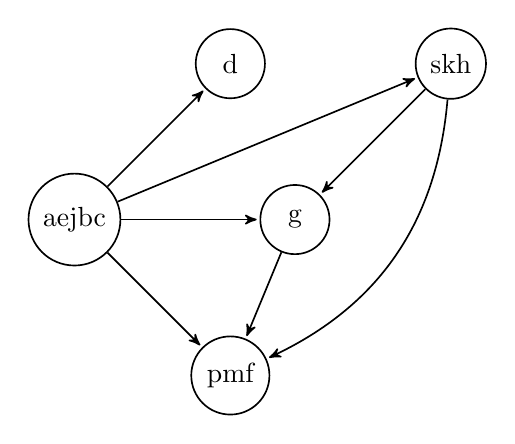
\begin{tikzpicture}[->,>=stealth',shorten >=1pt,auto,node distance=2.8cm,
                    semithick]
%  \tikzstyle{every state}=[fill=white,draw=none,text=black]

  \node[state]         (A)                                {aejbc};
  \node[state]         (D) [above right of=A] {d};
  \node[state]         (C) [below right of =A] {pmf};
  \node[state]         (G) [right of=A]          {g};
  \node[state]         (S) [above right of=G]  {skh};



  \path (A) edge node{} (D)
                  edge node{} (G)
                  edge node{} (C)
                  edge node{} (S)
           (S) edge node{} (G)
                 edge[bend left] node{} (C)
           (G) edge node{} (C)
;
\end{tikzpicture}


\section{Problem 2}
A binary tree is called a full binary tree if any internal node has exactly two children. Let L be the set of leaves in a full binary tree T. Use mathematical induction on the height of the tree to prove the following formula:
$ \sum\limits_{x \in L} \frac{1}{2^{depth(x)}} = 1 $.

\paragraph{Solution}
Assume that our tree is also complete.  Then for a tree with $n$ leaves, we have the height of the tree (and thus the depth to each leaf) as $\lg(n)$ giving: \\
\\
\centerline{$ \sum\limits_{x \in L} \frac{1}{2^{depth(x)}} = \frac{n}{2^{\lg(n)}} = \frac{n}{n} = 1 $}

So assume that our tree is full but not complete.  We will use induction to show the relationship.\\
Base Case: $n = 1$.  All we have is the root so: \\
\centerline{$ \sum\limits_{x \in L} \frac{1}{2^{depth(x)}} = \frac{1}{2^{\lg(1)}} = \frac{1}{2^0} = 1 $}

Inductive Step:
Now assume that $n>1$ and we will show the relationship. \\
Let $r$ be the number of nodes in the last row and $r'$ be the number of nodes in the (last - 1) row that are leaves.  Consider the subtree consisting of the root to the parents of these nodes.
This is a full tree with number of leaves equal to half of n and thus satisfies:\\
\centerline{$ \sum\limits_{x \in L_{Subtree}} \frac{1}{2^{depth(x)}}= 1 $}
We will parition the left sum into two sums, those nodes whose children are in $r$, define their set as $m$, and those nodes whose children are in $r'$, define their set as $m'$:\\
\centerline{$ \sum\limits_{x \in L_{Subtree}} \frac{1}{2^{depth(x)}}=  \sum\limits_{x \in m} \frac{1}{2^{depth(x)}} +  \sum\limits_{x \in m'} \frac{1}{2^{depth(x)}}  = 1 $}

Now, for each parent, we have 2 child nodes who are the leaves of the original tree which are one height greater than their parents, giving the formula for the original tree's leaves as:\\
\begin{align*}
\sum\limits_{x \in L} \frac{1}{2^{depth(x)}}  & =  \sum\limits_{x \in r} \frac{1}{2^{depth(x)}} +  \sum\limits_{x \in r'} \frac{1}{2^{depth(x)}} \\
                                                                         & = \sum\limits_{x \in m} \frac{2}{2^{depth(x)+1}} +  \sum\limits_{x \in m'} \frac{2}{2^{depth(x)+1}} \\
%                                                                         & = \frac{2m}{2^{\lg( \lceil(m+m') \rceil )+1}} + \frac{2m'}{2^{\lg( \lfloor (m +m' \rfloor )+1}} \\
 %                                                                        & = \frac{m}{2^{\lg(\lceil(m+m') \rceil)}} + \frac{m'}{2^{\lg( \lfloor (m +m' \rfloor)}} \\
                                                                         & =   \sum\limits_{x \in m} \frac{1}{2^{depth(x)}} +  \sum\limits_{x \in m'} \frac{1}{2^{depth(x)}} \\
                                                                         & = 1\\
\end{align*}


\section{Problem 3}
 Please write a program or a pseudo code that finds the successor for a given node x. 

\paragraph{Solution}
For this algorithm we begin by checking to see if we have a right child.  If we don't, and we are the root, then we are done.
Else, we see which side of the tree we are on by comparing ourselves with the root.\\
If we are on the right side with no right child, we look up the tree, looking for the closest father/grandfather/ancestor whose key value is greater than our nodes, signifying that it
is our successor.  If we reach the root, we do not have a successor.
\\
If we are on the left hand side, we do a similar thing, looking up the tree for the next key value whose value is greater than ours.  Except this time we are guaranteed to have a successor
as the root must greater than all the nodes on the left hand side.
\\
If we do have a right child, we then check to see if our right child has a left child, if not, he is our successor.  If so, we continue to check our left child for more left children until we reach a leaf.  That node is our successor.

\begin{lstlisting}
successor( tree t, node n)
{
	if( n.right() == nil && n.key() = t.root.key())
	{
		return nil \\no successor
	}
	else if( n.right() == nil && n.key() > t.root.key())
	{
		fatherR = n.father()
		while( fatherR.key != t.root.key())
		{
		 if( fatherR.key() > n.key() )
		 {
		  return fatherR.key()
		 }
		 else
		 {
		  fatherR = fatherR.father()
		 }
		}
		 return nil \\no successor 
	}
	else if( n.right() == nil && n.key() < t.root.key())
	{
		fatherL = n.father()
		while( true )
		{
		 if( fatherL.key() > n.key() )
		 {
		  return fatherL.key()
		 }
		 else
		 {
		  fatherL = fatherL.father()
		 }
		}
	}
	
	else
	{
		childR = n.right()
		if( childR.left() == nil)
		{
		 return childR.key()
		}
		successor = childR.left()
		while( successor.left() != nil)
		{
		 successor = successor.left()
		}
		return successor.key()
	}
}
\end{lstlisting}

\section{Problem 4}
Let G(V, E) be a weighted (undirected) graph G(V, E). The weight of an edge is called the width of the edge. Let P(u, v) be a path from vertex u to vertex v in graph G(V, E). The width of the path is defined to be the smallest weight among all edges on the path. (The edge with the smallest weight is called the bottle neck edge.) A path P(u, v) is called the widest if the width of the path is the largest among all paths from u to v. Please modify the Dijkstra’s algorithm to compute the widest path from a given vertex s to every other vertex. The correctness proof is not required. 


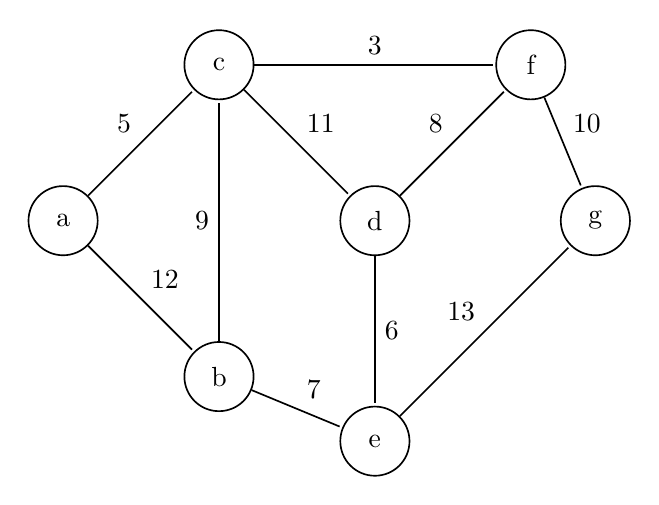
\begin{tikzpicture}[-,>=stealth',shorten >=1pt,auto,node distance=2.8cm,
                    semithick]
%  \tikzstyle{every state}=[fill=white,draw=none,text=black]

  \node[state]         (A)                                {a};
  \node[state]         (B) [below  right of=A] {b};
  \node[state]         (C) [above right of=A] {c};
  \node[state]         (D) [below right of=C] {d};
  \node[state]         (E) [below of=D]          {e};
  \node[state]         (F) [above right of=D]  {f};
  \node[state]         (G) [right of=D]       {g};

  \path (A) edge              node {12} (B)
                  edge              node {5} (C)
        (B) edge                  node {7} (E)
            edge                    node {9} (C)
        (C) edge                  node {11} (D)
            edge                    node {3} (F)
        (D) edge                  node {6} (E)
            edge                    node {8} (F)
        (E) edge                  node {13} (G)
         (F) edge                 node {10} (G);
\end{tikzpicture}

\paragraph{ Solution } 
To find the maximum width graph, we will employ Dijkstra's algorithm, but we will first take the inverse of all the edges weights.  Since Dijkstra's finds the smallest path, with the edges inverted, we will find the largest. \\
Also, similar to Prim's algorithm, we only need to add the node with the shortest (which represents the longest) distance from the tree. 

\begin{lstlisting}
WidestPath( G, w, s)
{
 //invert each weight
 for each weight in w
 {
  weight = 1/weight
 }
 
 //then just do Dijkstra's as normal
 for each vertex in G
 {
  d[v] = infinity
  p[v] = nil
 }
 d[s] = 0
 S = empty
 Q = V[G]
 while Q nonempty
 {
  u = Extract-Min( Q )
  S = S U {u}
  for each vertex adjacent to u
  {
   if(d[v] > w(u,v))
   {
    d[v] = w(u,v)
	p[v] = u
   }
  }
 }
}

\end{lstlisting}

To print the path from $s$ to $v$ we merely have to recursively print out $v$, change v to it's father, and continue until we are at $s$ which has not father.
\\
We will now show how this is done on the example.
Our initialized graph:\\
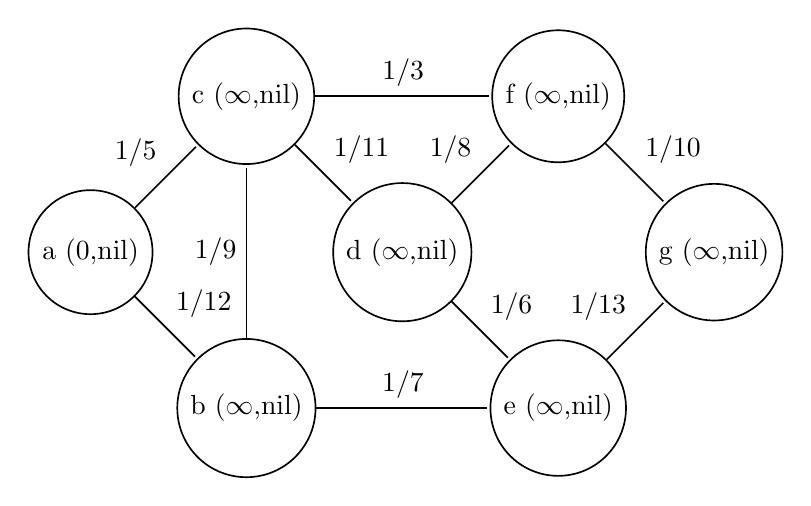
\begin{tikzpicture}[-,>=stealth',shorten >=1pt,auto,node distance=2.8cm,
                    semithick]
%  \tikzstyle{every state}=[fill=white,draw=none,text=black]

  \node[state]         (A)                                {a (0,nil)};
  \node[state]         (B) [below  right of=A] {b ($\infty$,nil)};
  \node[state]         (C) [above right of=A] {c ($\infty$,nil)};
  \node[state]         (D) [below right of=C] {d ($\infty$,nil)};
  \node[state]         (E) [below right of=D]          {e ($\infty$,nil)};
  \node[state]         (F) [above right of=D]  {f ($\infty$,nil)};
  \node[state]         (G) [above right of=E]       {g ($\infty$,nil)};

  \path (A) edge              node {1/12} (B)
                  edge              node {1/5} (C)
        (B) edge                  node {1/7} (E)
            edge                    node {1/9} (C)
        (C) edge                  node {1/11} (D)
            edge                    node {1/3} (F)
        (D) edge                  node {1/6} (E)
            edge                    node {1/8} (F)
        (E) edge                  node {1/13} (G)
         (F) edge                 node {1/10} (G);
\end{tikzpicture}


We start with $a$ and look at it's neighbors, since they both have widths than their current values we update them.\\
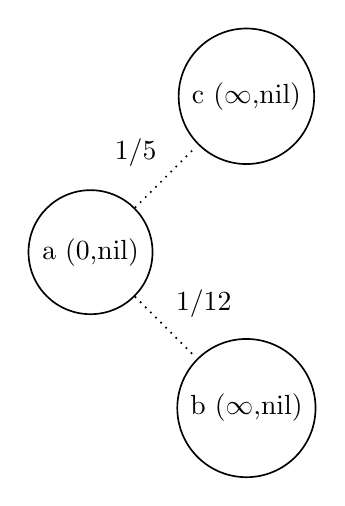
\begin{tikzpicture}[-,>=stealth',shorten >=1pt,auto,node distance=2.8cm,
                    semithick]
%  \tikzstyle{every state}=[fill=white,draw=none,text=black]

  \node[state]         (A)                                {a (0,nil)};
  \node[state]         (B) [below  right of=A] {b ($\infty$,nil)};
  \node[state]         (C) [above right of=A] {c ($\infty$,nil)};


  \path (A) edge [dotted]             node {1/12} (B)
                  edge [dotted]             node {1/5} (C);

\end{tikzpicture}


We now have 2 choices we could make, $c$ or $b$.  We choose $b$ as it has the smallest width.  \\
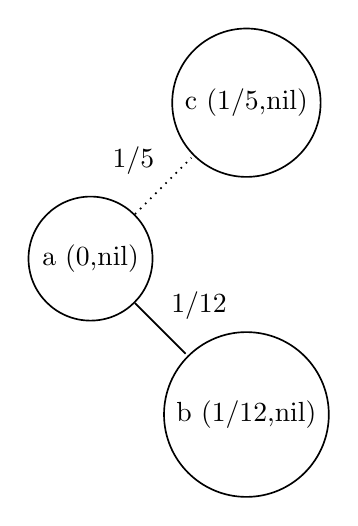
\begin{tikzpicture}[-,>=stealth',shorten >=1pt,auto,node distance=2.8cm,
                    semithick]
%  \tikzstyle{every state}=[fill=white,draw=none,text=black]

  \node[state]         (A)                                {a (0,nil)};
  \node[state]         (B) [below  right of=A] {b (1/12,nil)};
  \node[state]         (C) [above right of=A] {c (1/5,nil)};


  \path (A) edge              node {1/12} (B)
                  edge [dotted]             node {1/5} (C);

\end{tikzpicture}

We continue, we look at the neighbors of $b$ and update $c$ as their edge is smaller, same with $e$. \\

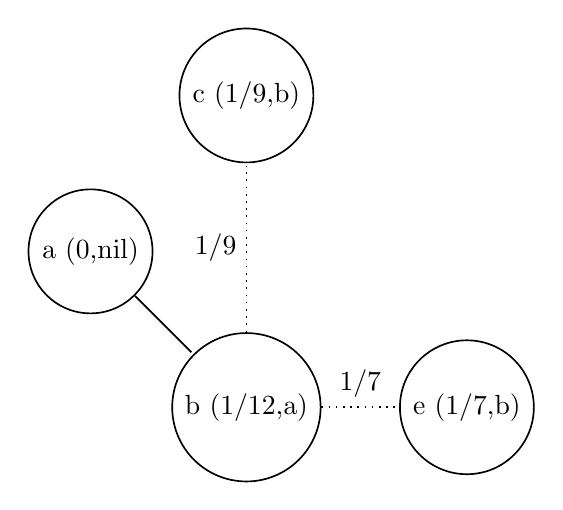
\begin{tikzpicture}[-,>=stealth',shorten >=1pt,auto,node distance=2.8cm,
                    semithick]
%  \tikzstyle{every state}=[fill=white,draw=none,text=black]

  \node[state]         (A)                                {a (0,nil)};
  \node[state]         (B) [below  right of=A] {b (1/12,a)};
  \node[state]         (C) [above right of=A] {c (1/9,b)};
  \node[state]         (E) [right of =B]          {e (1/7,b)};


  \path (A) edge           node {} (B)
               
             (B) edge [dotted]                 node {1/7} (E)
                   edge[dotted]                    node {1/9} (C);

\end{tikzpicture}

We choose $c$ and look at it's neighbors and update them.

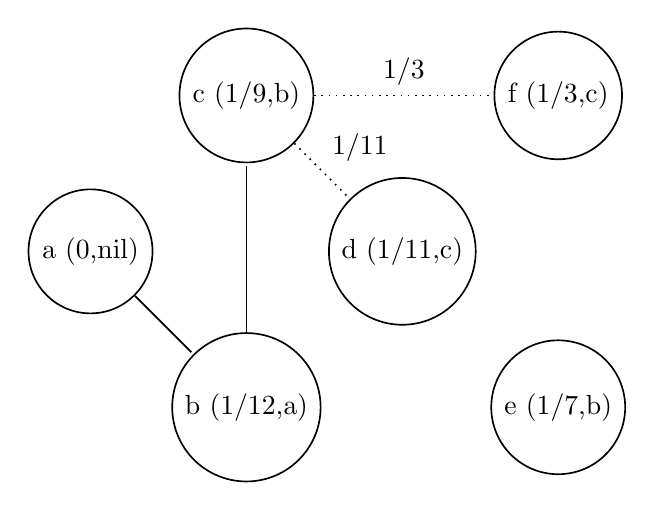
\begin{tikzpicture}[-,>=stealth',shorten >=1pt,auto,node distance=2.8cm,
                    semithick]
%  \tikzstyle{every state}=[fill=white,draw=none,text=black]

  \node[state]         (A)                                {a (0,nil)};
  \node[state]         (B) [below  right of=A] {b (1/12,a)};
  \node[state]         (C) [above right of=A] {c (1/9,b)};
  \node[state]         (D) [below right of=C] {d (1/11,c)};
  \node[state]         (E) [below right of=D]          {e (1/7,b)};
  \node[state]         (F) [above right of=D]  {f (1/3,c)};


  \path (A) edge           node {} (B)
                 
             (B) 
                   edge              node {} (C)
 (C) edge [dotted]                 node {1/11} (D)
            edge  [dotted]                  node {1/3} (F);

\end{tikzpicture}

We choose $d$ and update it's neighbors. \\

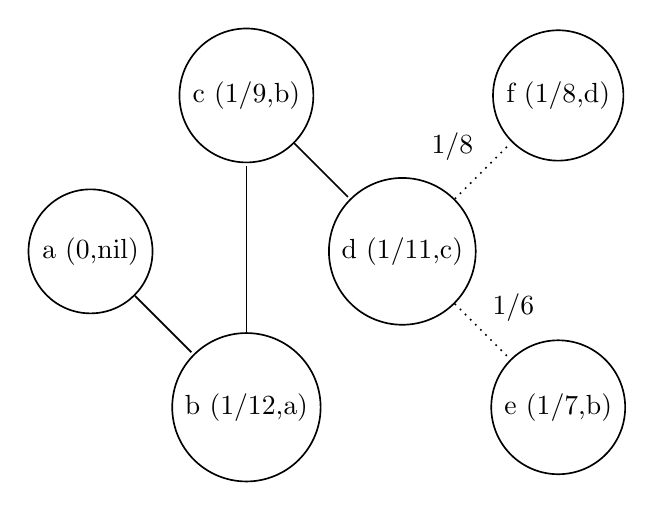
\begin{tikzpicture}[-,>=stealth',shorten >=1pt,auto,node distance=2.8cm,
                    semithick]
%  \tikzstyle{every state}=[fill=white,draw=none,text=black]

  \node[state]         (A)                                {a (0,nil)};
  \node[state]         (B) [below  right of=A] {b (1/12,a)};
  \node[state]         (C) [above right of=A] {c (1/9,b)};
  \node[state]         (D) [below right of=C] {d (1/11,c)};
  \node[state]         (E) [below right of=D]          {e (1/7,b)};
  \node[state]         (F) [above right of=D]  {f (1/8,d)};


  \path (A) edge           node {} (B)
                
             (B)
                   edge              node {} (C)
 (C) edge                  node {} (D)
           
 (D) edge   [dotted]               node {1/6} (E)
            edge   [dotted]                 node {1/8} (F);

\end{tikzpicture}

We chose $f$ and update it's neighbors. \\

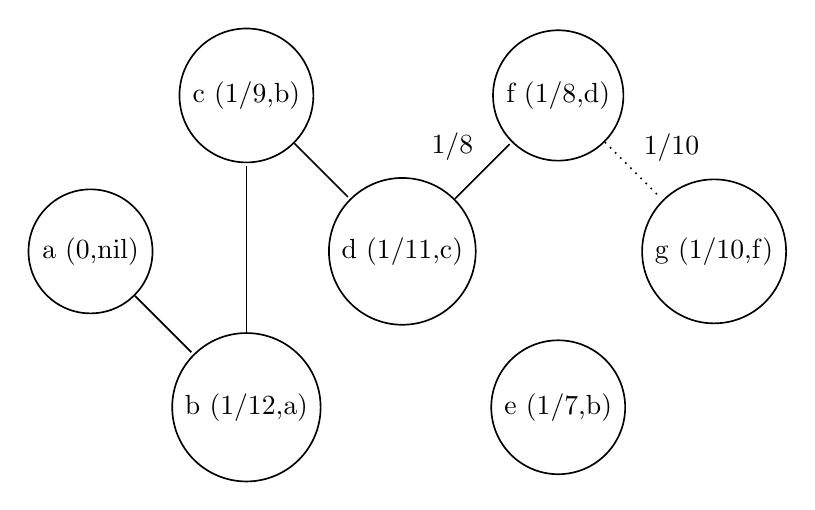
\begin{tikzpicture}[-,>=stealth',shorten >=1pt,auto,node distance=2.8cm,
                    semithick]
%  \tikzstyle{every state}=[fill=white,draw=none,text=black]

  \node[state]         (A)                                {a (0,nil)};
  \node[state]         (B) [below  right of=A] {b (1/12,a)};
  \node[state]         (C) [above right of=A] {c (1/9,b)};
  \node[state]         (D) [below right of=C] {d (1/11,c)};
  \node[state]         (E) [below right of=D]          {e (1/7,b)};
  \node[state]         (F) [above right of=D]  {f (1/8,d)};
  \node[state]         (G) [above right of=E]       {g (1/10,f)};

  \path (A) edge           node {} (B)
                
             (B) 
                   edge              node {} (C)
 (C) edge                  node {} (D)
            
 (D) 
            edge                    node {1/8} (F)
(F) edge [dotted]                 node {1/10} (G);

\end{tikzpicture}

We choose $g$ and update it's neighbor. \\

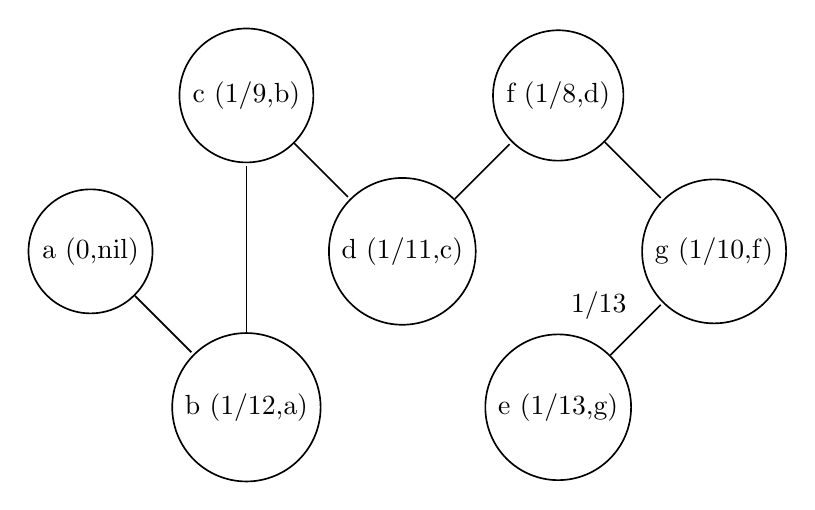
\begin{tikzpicture}[-,>=stealth',shorten >=1pt,auto,node distance=2.8cm,
                    semithick]
%  \tikzstyle{every state}=[fill=white,draw=none,text=black]

  \node[state]         (A)                                {a (0,nil)};
  \node[state]         (B) [below  right of=A] {b (1/12,a)};
  \node[state]         (C) [above right of=A] {c (1/9,b)};
  \node[state]         (D) [below right of=C] {d (1/11,c)};
  \node[state]         (E) [below right of=D]          {e (1/13,g)};
  \node[state]         (F) [above right of=D]  {f (1/8,d)};
  \node[state]         (G) [above right of=E]       {g (1/10,f)};

  \path (A) edge           node {} (B)
                  
             (B) 
                   edge              node {} (C)
 (C) edge                  node {} (D)
            
 (D) 
            edge                    node {} (F)
(E) edge                  node {1/13} (G)
(F) edge                  node {} (G);

\end{tikzpicture}

We choose $e$ and we have no neighbors not visited and so are done.



\section{Problem 5}
Let T be a maximum spanning tree of graph G(V, E). Prove that any path P(u, v) in T is the widest path between u and v in G, where u, v can be any two vertices in G. 
\paragraph{ Solution }
Assume, by contradiction that P(u,v) is not the widest path from $u$ to $v$.  Then $\exists P'(u,v)$ such that $wid(P'(u,v)) > wid(P(u,v))$. \\
This  means that $\exists (x,y) \in P(u,v)$ such that $weight (x,y) < (x',y') ~~\forall ~~ (x',y') \in P'(u,v)$. \\
There must also be an edge in $P'(u,v)$ that is not in our maximum spanning tree, else we would have two paths from $u$ to $v$ and thus a cycle and
our tree wouldn't be a spanning tree.\\
We will construct a tree as follows:\\
Take our maximum spanning tree and remove $(x,y)$. This will form two seperate trees.\\
We will rejoin the trees by selecting an edge from $P'(u,v)$ that joins them.  This edge must exist as the path $P'(u,v)$ exists.  This will also form a spanning tree as
 it connects the two disjoint trees.  Call this edge $(x',y')$.\\
So it follows that $ \sum\limits_{weights} T_{new} > \sum\limits_{weights} T_{old}$ as they are exactly the same except for $(x,y)$ in $T_{old}$ and $(x',y')$ in $T_{new}$ and
$(x,y) < (x',y')$.



\end{document}